\documentclass[letterpaper,openany,oneside,twocolumn]{book}

\newcommand{\PATH}{../../../../../../}

\usepackage{\PATH templates/utilities/m4rz-fonts}
\usepackage{\PATH templates/utilities/m4rz-colors}

\usepackage[justified]{\PATH templates/template_dnd/dnd}

\graphicspath{{../images}}
% --------------------------------------------------------------------------------------------------------------- %
% #+#+#+#+#+#+#+#+#+#+#+#+#+#+#+#+#+#+#+#+#  CHARACTER-SHEET  TEMPLATE  #+#+#+#+#+#+#+#+#+#+#+#+#+#+#+#+#+#+#+#+# %
% --------------------------------------------------------------------------------------------------------------- %
% Edition and Backend can be specified when loading the character-sheet template:

%% edition = { pre5e24 /  5e24 }
%%% Layout of the Character Information and Spell Sheet are set to the specified version
%%% The background sheet is always based on the pre5e24 version
%%% The spell sheet of the pre5e24 can always be accessed via "\renderoldspellsheet" to hold more spells

%% backend = { postscript / tikz }
%%% Using TikZ may lead to faster compilation times on some machines
%%% The character sheet of the pre5e24 edition is still using PostScript (WIP)
\usepackage[edition=5e24, backend=tikz]{\PATH templates/template_character-sheet/character-sheet-stylesheet}
\usepackage{\PATH templates/template_magic-item/magic-items_commands}
\usepackage{\PATH templates/template_resource/resource_commands}

\setlength\oddsidemargin{\dimexpr(\paperwidth-\textwidth)/2 - 1in\relax}
\setlength\evensidemargin{\oddsidemargin}

% --------------------------------------------------------------------------------------------------------------- %
% #+#+#+#+#+#+#+#+#+#+#+#+#+#+#+#+#+#+#+#+#+#  CHARACTER INFORMATION  #+#+#+#+#+#+#+#+#+#+#+#+#+#+#+#+#+#+#+#+#+# %
% --------------------------------------------------------------------------------------------------------------- %
\CharacterName{Luna Finn}
\PlayerName{M4RZ-Crafting} % Player Name is only displayed in the pre5e24 edition

\Class{Druid}
\Subclass{Circle of the Shepherd}
\Background{Farmer}
\Race{Satyr}
%% Multiclass
%\MultiClassMainLevel{2}
%\MultiClass{Warlock}

\Level{4} % Automatically sets XP and Proficiency Bonus
% --------------------------------------------------------------------------------------------------------------- %
% #+#+#+#+#+#+#+#+#+#+#+#+#+#+#+#+#+#+#+#+#+#+#+# ABILITY  SCORES #+#+#+#+#+#+#+#+#+#+#+#+#+#+#+#+#+#+#+#+#+#+#+# %
% --------------------------------------------------------------------------------------------------------------- %
% UNMODIFIED ABILITY SCORES
% Modifiers, Saving Throws and Skills are calculated automatically
\StrengthRolledScore{9}
\DexterityRolledScore{14}
\ConstitutionRolledScore{15}
\IntelligenceRolledScore{12}
\WisdomRolledScore{16}
\CharismaRolledScore{12}

% SCORE MODIFIERS (ASI, Background and Race Boni)
\StrengthScoreBonus{0}
\DexterityScoreBonus{1}		% Speedy Feat
\ConstitutionScoreBonus{1}	% Farmer Background
\IntelligenceScoreBonus{0}
\WisdomScoreBonus{2}		% Farmer Background
\CharismaScoreBonus{0}

\calculateAbilityScores{}

% ABILITY MODIFIERS BONUS (Bonus to modifiers without adjusting the Score)
\StrengthModifierBonus{0}
\DexterityModifierBonus{0}
\ConstitutionModifierBonus{0}
\IntelligenceModifierBonus{0}
\WisdomModifierBonus{0}
\CharismaModifierBonus{0}
% --------------------------------------------------------------------------------------------------------------- %
% #+#+#+#+#+#+#+#+#+#+#+#+#+#+#+#+#+#+#+#+# PROFICIENCIES AND EXPERTISE #+#+#+#+#+#+#+#+#+#+#+#+#+#+#+#+#+#+#+#+# %
% --------------------------------------------------------------------------------------------------------------- %
% SAVING THROWS {Proficient = P, Experties = E}
\StrengthProficiency{}
\DexterityProficiency{}
\ConstitutionProficiency{}
\IntelligenceProficiency{P}
\WisdomProficiency{P}
\CharismaProficiency{}

%% Bonus to only Saving Throw (i.e. Ring of Protection)
\StrengthSavingThrowBonus{0}
\DexteritySavingThrowBonus{0}
\ConstitutionSavingThrowBonus{0}
\IntelligenceSavingThrowBonus{0}
\WisdomSavingThrowBonus{0}
\CharismaSavingThrowBonus{0}

\calculateScoreModifiersAndSavingThrows{}

% SKILL PROFICIENCY
% \SkillProficiency[#1]{#2}
%%	#1 = Bonus to this Skill (i.e. Stone of Good Luck)
%%	#2 = {Proficient = P, Experties = E}
%% STRENGTH SKILLS
\AthleticsProficiency{}

%% DEXTERITY SKILLS
\AcrobaticsProficiency{}
\SleightOfHandProficiency{}
\StealthProficiency{}

%% INTELLIGENCE SKILLS
\ArcanaProficiency[\calculateModifier{\WisdomScoreValue}]{} % Primal Order - Magician + WIS mod
\HistoryProficiency{}
\InvestigationProficiency{}
\NatureProficiency[\calculateModifier{\WisdomScoreValue}]{P} % Primal Order - Magician + WIS mod
\ReligionProficiency{P}

%% WISDOM SKILLS
\AnimalHandlingProficiency{P}
\InsightProficiency{}
\MedicineProficiency{}
\PerceptionProficiency{}
\SurvivalProficiency{P}

%% CHARISMA SKILLS
\DeceptionProficiency{}
\IntimidationProficiency{}
\PerformanceProficiency{P}
\PersuasionProficiency{P}

% ABILITY MODIFIERS BONUS
\StrengthModifierBonus{0}
\DexterityModifierBonus{0}
\ConstitutionModifierBonus{0}
\IntelligenceModifierBonus{0}
\WisdomModifierBonus{0}
\CharismaModifierBonus{0}

%\JackOfAllTrades{1} % Adds half Proficiency Bonus to each Skill and Initiative
\calculateAllSkillModifiers{}
% --------------------------------------------------------------------------------------------------------------- %
% #+#+#+#+#+#+#+#+#+#+#+#+#+#+#+#+#+#+#+#+#+#+#+# CHARACTER STATS #+#+#+#+#+#+#+#+#+#+#+#+#+#+#+#+#+#+#+#+#+#+#+# %
% --------------------------------------------------------------------------------------------------------------- %
% HEROIC INSPIRATION
\Inspiration{}

% INITIATIVE MODIFIER
\InitiativeModifier{0}

% SPEED
\Speed{45}

% SIZE
\Size{Medium}

% PASSIVE PERCEPTION
\PassivePerceptionModifier{0}

% ARMOR CLASS (\Equip Shield does not adjust AC-Value)
\EquipShield
\ArmorClass{\intcalcAdd{11}{\intcalcAdd{1}{\calculateModifier{\DexterityScoreValue}}}}

% HIT POINTS
\ToughFeat{1} % Automatic Tough Feat Integration
\MaxHitPointsRolled{29} % Without Constitution Bonus, is added automatically
\CurrentHitPoints{\MaxHitPointsValue}
\TemporaryHitPoints{}
\HitDice{d8}
\HitDiceSpent{0}
%% Multiclass
%\MultiClassHitDice{d10}
%\MultiClassHitDiceSpent{0}

% EQUIPMENT TRAINING AND PROFICIENCIES
%% ARMOR {Proficient = P}
\LightArmor{P}
\MediumArmor{}
\HeavyArmor{}
\Shields{P}

\WeaponsProficiency{Simple Weapons}
\ToolsProficiency{Carpenter's Tools, Herbalism Kit, Pan Flute}
% --------------------------------------------------------------------------------------------------------------- %
% #+#+#+#+#+#+#+#+#+#+#+#+#+#+#+#+#+#+#+#+# WEAPONS AND DAMAGE CANTRIPS #+#+#+#+#+#+#+#+#+#+#+#+#+#+#+#+#+#+#+#+# %
% --------------------------------------------------------------------------------------------------------------- %
% WEAPONS
% \addWeaponStatistic{#1}{#2}{#3}{#4}{#5}{#6}{#7}
%%	#1 = Name of Weapon
%%	#2 = Handle (usually Playername, but arbitrary)
%%	#3 = Attack-Skill (STR, DEX, INT, WIS, CHA)
%%	#4 = Proficiency (proficient = P, expertise = E)
%%	#5 = Bonus Attack Modifier (i.e. Weapon +1)
%%	#6 = Damage + Damage Type
%%	#7 = Notes
\addWeaponStatistic{Quarterstaff}{LunaFinn}{STR}{P}{0}{1d6 b}{versatile (1d8)}
\addWeaponStatistic{Sickle}{LunaFinn}{STR}{P}{0}{1d4 s}{light}
% UNARMED STRIKE
\addWeaponStatistic{Unarmed Strike}{LunaFinn}{STR}{P}{0}{1d6 b}{}
% DAMAGE CANTRIPS
% \addSpellStatistic{#1}{#2}{#3}{#4}{#5}
%%	#1 = Name of Spell
%%	#2 = Attack Modifier or DC {ATK, DC, BOTH}
%%	#3 = Skill (i.e. \calculateModifier{\IntelligenceScoreValue})
%%	#6 = Damage
%%	#7 = Notes
\addSpellStatistic{Primal Savagery}{ATK}{\calculateModifier{\WisdomScoreValue}}{1d10}{Acid, melee}
% --------------------------------------------------------------------------------------------------------------- %
% #+#+#+#+#+#+#+#+#+#+#+#+#+#+#+#+#+#+#+#+#+#+# FEATURES AND TRAITS #+#+#+#+#+#+#+#+#+#+#+#+#+#+#+#+#+#+#+#+#+#+# %
% --------------------------------------------------------------------------------------------------------------- %
% Action = A, Bonus Action = B, Reaction = R, Limited Use = L
% \CustomItemLabel{#1} can be used in nested itemize environments to access labels for Action, Bonus Action etc.
% CLASS FEATURE
\AddClassFeature{E}{\textbf{Primal Order - Magician}\\Nature and Arcana Skill Bonus (Wisdom Modifier)}
\AddClassFeature{L}{\textbf{Wild Shape}\\2 per Long Rest}
\AddClassFeature{L}{\textbf{Wild Companion}}
\AddClassFeature{E}{\textbf{Speech of the Woods}\\Communicate with Beasts}
\AddClassFeature{B}{\textbf{Spirit Totem}\\1 per SR/LR}
% SPECIES TRAITS
\AddSpeciesFeature{E}{\textbf{Ram}\\1d6 + STR Unarmed Strike}
\AddSpeciesFeature{E}{\textbf{Magic Resistance}\\Advantage on Saving Throws against Spells}
\AddSpeciesFeature{E}{\textbf{Mirthful Leaps}\\+1d8 feet jump distance/height}
% FEATS
\AddFeat{\textbf{Speedy}}
\AddFeat{\textbf{Tough}}
% --------------------------------------------------------------------------------------------------------------- %
% #+#+#+#+#+#+#+#+#+#+#+#+#+#+#+#+#+#+#+#+#+# BACKGROUND & APPEARANCE #+#+#+#+#+#+#+#+#+#+#+#+#+#+#+#+#+#+#+#+#+# %
% --------------------------------------------------------------------------------------------------------------- %
% APPEARANCE
\Age{}
\Height{}
\Weight{}
\Eyes{}
\Skin{}
\Hair{}
\CharacterAppearance{horizontal} % (vertical/horizontal/none)
	{0} % Main-Text Offset (Steps of 15.75 [equal to line-height])
	{0} % Picture X-Shift (absolute value, no effect in vertical mode)
	{0} % Picture Y-Shift (absolute value)
	{Shepherd_Druid.png} % Description without Picture
	{{\ }{\ }} % Description with Picture

% ORGANIZATION & ALLIES
\OrganizationName{Eagle Druids of Crail}
\OrganizationSymbol{Eagle_Druids_of_Crail.png}
\AlliesAndOrganizations{
	The Eagle Druids of Crail are a revered circle tasked with the sacred duty of hatching, nurturing, and bonding with the majestic Great Eagles of Crail. Nestled within the windswept cliffs of Fledgling's Cove, they live in harmony with the colossal raptors, guiding them with ancient rites and druidic magic. To be chosen as one of their number is a rare honour, marking one as a guardian of Crail's skies and a spiritual link between the city and its soaring protectors. Their wisdom and prestige echo far beyond the citadel walls, earning them respect throughout the Kingdom of Fife. 
}{\ }

% ADDITIONAL FEATURES & TRAITS
\AdditionalFeaturesAndTraits{
	\ 
}

% BACKGROUND
\Characterbackground{
	\ 
}

% TREASURES
\Treasure{
	\ 
}
% --------------------------------------------------------------------------------------------------------------- %
% #+#+#+#+#+#+#+#+#+#+#+#+#+#+#+#+# SPELLS, PERSONALITY  TRAITS  AND  EQUIPMENT #+#+#+#+#+#+#+#+#+#+#+#+#+#+#+#+# %
% --------------------------------------------------------------------------------------------------------------- %
% #+#+#+#+#+#+#+#+#+#+#+#+#+#+#+#+#+#+#+#+#+#+# PERSONALITY  TRAITS #+#+#+#+#+#+#+#+#+#+#+#+#+#+#+#+#+#+#+#+#+#+# %
% --------------------------------------------------------------------------------------------------------------- %
\PersonalityTraits{
	\ 
}
\Alignment{Lawful Good}

\Ideals{
	\ 
}

\Bonds{
	\ 
}

\Flaws{
	\ 
}

% LANGUAGES
\Languages{Common, Druidic, Dwarvish, Sylvan}
% --------------------------------------------------------------------------------------------------------------- %
% #+#+#+#+#+#+#+#+#+#+#+#+#+#+#+#+#+#+#+#+#+#+#+#+#  EQUIPMENT  #+#+#+#+#+#+#+#+#+#+#+#+#+#+#+#+#+#+#+#+#+#+#+#+# %
% --------------------------------------------------------------------------------------------------------------- %
\Equipment{
	Quarterstaff, 2 Sickles, Leather Armor +1, Shield\\
	\textbf{Golden Feather (Druidic Focus)}, Gilded Acorn (200GP), Carpenter's Kit, Healer's Kit, Herbalism Kit\\
	backpack, bedroll, 2 flasks of oil, 10 days of rations, tinderbox, 10 torches, waterskin, 50 ft. of hempen rope
}
%% Attuned Magic Items (Max 3, every other is ignored)
%\addAttunedMagicItem{}
%% Gold
\CP{}
\SP{}
\EP{}
\GP{}
\PP{}
% --------------------------------------------------------------------------------------------------------------- %
% #+#+#+#+#+#+#+#+#+#+#+#+#+#+#+#+#+#+#+#+#+#+#+#+#+#  SPELL  #+#+#+#+#+#+#+#+#+#+#+#+#+#+#+#+#+#+#+#+#+#+#+#+#+# %
% --------------------------------------------------------------------------------------------------------------- %
% SPELLCASTING STATS
\SpellcastingClass{Druid}
\SpellcastingAbility{WIS} % STR, DEX, CON, INT, WIS, CHA
\SpellSaveDCModifier{0} % any modifier that isn't contained in "8 + Ability Modifier + Proficiency Bonus"
\SpellAttackModifier{0} % any modifier that isn't contained in "Ability Modifier + Proficiency Bonus"
%% Calculate Modifier, DC, and Attack Bonus
\CalculateSpellStatistics{}

% SPELL SLOTS
\FirstLevelSpellSlotsTotal{4}
\SecondLevelSpellSlotsTotal{3}

% ADD SPELLS
% \addPreparedSpell{#1}{#2}{#3}{#4}{#5}{#6}{#7}{#8}{#9}
%%	#1 = Spell-Level { 0 - 9 }
%%	#2 = Spell Name
%%	#3 = Casting Time
%%	#4 = Range
%%	#5 = Concentration {T}
%%	#6 = Ritual {T}
%%	#7 = Required Material {T}
%%	#8 = Notes
%%	#9 = All Spell Components (for old spell sheet)

% \AddSpell{#1}{#2}{#3}{#4} (Adds spell only to old spell sheet)
%%	#1 = Spell-Level { 0 - 9 }
%%	#2 = Spell Prepared {True, False}
%%	#3 = Spell Name
%%	#4 = Spell Components {V, S, M}

%! If the maximum number of spells that can be displayed is exceeded a warning is added to the log and the spell is ommitted from being displayed !%
\addPreparedSpell{0}
	{Guidance}
	{Action}
	{Touch}
	{T}
	{}
	{}
	{V, S}
	{V, S}
\addPreparedSpell{0}
	{Gust}
	{Action}
	{30 Feet}
	{}
	{}
	{}
	{V, S}
	{V, S}
\addPreparedSpell{0}
	{Mold Earth}
	{Action}
	{30 Feet}
	{}
	{}
	{}
	{S}
	{S}
\addPreparedSpell{0}
	{Primal Savagery}
	{Action}
	{Self}
	{}
	{}
	{}
	{S}
	{S}
\addPreparedSpell{1}
	{Animal Friendship}
	{Action}
	{30 Feet}
	{}
	{}
	{T}
	{V, S}
	{V, S, M}
\addPreparedSpell{1}
	{Beast Bond}
	{Action}
	{Touch}
	{T}
	{}
	{T}
	{V, S}
	{V, S, M}
\addPreparedSpell{1}
	{Cure Wounds}
	{Action}
	{Touch}
	{}
	{}
	{}
	{V, S}
	{V, S}
\addPreparedSpell{1}
	{Faerie Fire}
	{Action}
	{60 Feet}
	{T}
	{}
	{}
	{V}
	{V}
\addPreparedSpell{2}
	{Dust Devil}
	{Action}
	{60 Feet}
	{T}
	{}
	{T}
	{V, S}
	{V, S, M}
\addPreparedSpell{2}
	{Summon Beast}
	{Action}
	{90 Feet}
	{T}
	{}
	{T}
	{V, S}
	{V, S, M}
\addPreparedSpell{2}
	{Warding Wind}
	{Action}
	{Self}
	{T}
	{}
	{}
	{V}
	{V}
% --------------------------------------------------------------------------------------------------------------- %
% #+#+#+#+#+#+#+#+#+#+#+#+#+#+#+#+#+#+#+#+#+#+#+# DOCUMENT  START #+#+#+#+#+#+#+#+#+#+#+#+#+#+#+#+#+#+#+#+#+#+#+# %
% --------------------------------------------------------------------------------------------------------------- %
\begin{document}

\newgeometry{left=0cm,right=0cm,top=0cm,bottom=0cm}
\onecolumn


% CHARACTER PAGE
\rendercharactersheet

% BACKSTORY PAGE
\renderbackgroundsheet

% SPELLCASTING PAGE
\renderspellsheet


\restoregeometry
\twocolumn

\chapter*{Features, Magic Items and Spells}

\section*{Satyr Traits}
\subsection*{Ram}
You can use your head and horns to make unarmed strikes. When you hit with them, the strike deals 1d6 + your Strength modifier bludgeoning damage, instead of the bludgeoning damage normal for an unarmed strike.
\subsection*{Magic Resistance}
You have advantage on saving throws against spells.
\subsection*{Mirthful Leaps}
Whenever you make a long jump or a high jump, you can roll a d8 and add the number rolled to the number of feet you cover, even when making a standing jump. This extra distance costs movement as normal.
\subsection*{Reveler}
As an embodiment of revelry, you have proficiency in the Performance and Persuasion skills, and you have proficiency with one musical instrument of your choice.

\section*{Feat}
\subsection*{Speedy}
You gain the following benefits.
\paragraph*{Dash over Difficult Terrain} When you take the Dash action on your turn, Difficult Terrain doesn't cost extra movement for the rest of the turn.
\paragraph*{Agile Movement} Opportunity Attacks have Disadvantage against you.
\subsection*{Tough}
Your Hit Point maximum increases by an amount equal to twice your character level when you gain this feat. Whenever you gain a character level thereafter, your Hit Point maximum increases by an additional 2 Hit Points.

\section*{Druid Traits}
\subsection*{Primal Order - Magician}
\textbf{Bonus:} \calculateModifier{\WisdomScoreValue}\\
You know one extra cantrip from the Druid spell list. In addition, your mystical connection to nature gives you a bonus to your Intelligence (Arcana or Nature) checks. The bonus equals your Wisdom modifier (minimum bonus of +1)
\subsection*{Wild Shape}
As a Bonus Action, you shape-shift into a Beast form that you have learned for this feature (Brown Bear, Giant Octopus, Ice Spider, Tiger). You stay in that form for a number of hours equal to half your Druid level or until you use Wild Shape again, have the Incapacitated condition, or die. You can also leave the form early as a Bonus Action.
\paragraph*{Rules While Shape-Shifted} While in a form, you retain your personality, memories, and ability to speak, and the following rules apply:
\subparagraph*{Temporary Hit Points} You gain a number of Temporary Hit Points equal to your Druid level. \textbf{(\intcalcMul{1}{\LevelValue} Temporary HP)}
\subparagraph*{Game Statistics} Your game statistics are replaced by the Beast's stat block, but you retain your creature type; Hit Points; Hit Point Dice; Intelligence, Wisdom, and Charisma scores; class features; languages; and feats. You also retain your skill and saving throw proficiencies and use your Proficiency Bonus for them, in addition to gaining the proficiencies of the creature. If a skill or saving throw modifier in the Beast's stat blocks higher than yours, use the one in the stat block.
\subparagraph*{No Spellcasting} You can't cast spells, but shapeshifting doesn't break your Concentration or otherwise interfere with a spell you've already cast.
\subparagraph*{Objects} Your ability to handle objects is determined by the form's limbs rather than your own. In addition, you choose whether your equipment falls in your space, merges into your new form, or is worn by it. Worn equipment functions as normal, but the DM decides whether it's practical for the new form to wear a piece of equipment based on the creature's size and shape. Your equipment doesn't change size or shape to match the new form, and any equipment that the new form can't wear must either fall to the ground or merge with the form. Equipment that merges with the form has no effect while you're in that form.
\subsection*{Wild Companion}
You can summon a nature spirit that assumes an animal form to aid you. As a Magic action, you can expend a spell slot or a use of Wild Shape to cast the Find Familiar spell without Material Components.

When you cast the spell in this way, the familiar is Fey and disappears when you finish a Long Rest.
\subsection*{Circle of the Shepherd}
\subsubsection*{Speech of the Woods}
You learn to speak, read, and write Sylvan. In addition, beasts can understand your speech, and you gain the ability to decipher their noises and motions. Most beasts lack the intelligence to convey or understand sophisticated concepts, but a friendly beast could relay what it has seen or heard in the recent past. This ability doesn't grant you any special friendship with beasts, though you can combine this ability with gifts to curry favor with them as you would with any nonplayer character.
\subsubsection*{Spirit Totem}
As a bonus action, you can magically summon an incorporeal spirit to a point you can see within 60 feet of you. The spirit creates an aura in a 30-foot radius around that point. It counts as neither a creature nor an object, though it has the spectral appearance of the creature it represents. As a bonus action, you can move the spirit up to 60 feet to a point you can see.

The spirit persists for 1 minute. Once you use this feature, you can't use it again until you finish a short or long rest.

The effect of the spirit's aura depends on the type of spirit you summon from the options below.

\paragraph*{Bear Spirit} The bear spirit grants you and your allies its might and endurance. Each creature of your choice in the aura when the spirit appears gains temporary hit points equal to 5 + your druid level. In addition, you and your allies gain advantage on Strength checks and Strength saving throws while in the aura.

\paragraph*{Hawk Spirit} The hawk spirit is a consummate hunter, aiding you and your allies with its keen sight. When a creature makes an attack roll against a target in the spirit's aura, you can use your reaction to grant advantage to that attack roll. In addition, you and your allies have advantage on Wisdom (Perception) checks while in the aura.

\paragraph*{Unicorn Spirit} The unicorn spirit lends its protection to those nearby. You and your allies gain advantage on all ability checks made to detect creatures in the spirit's aura. In addition, if you cast a spell using a spell slot that restores hit points to any creature inside or outside the aura, each creature of your choice in the aura also regains hit points equal to your druid level.

\section*{Spells}
\subsection*{Cantrip}

\DndSpellHeader
  {Guidance}
  {Divination Cantrip}
  {Action}
  {Touch}
  {V, S}
  {Concentration, Up to 1 Minute}

You touch one willing creature. Once before the spell ends, the target can roll a d4 and add the number rolled to one ability check of its choice. It can roll the die before or after making the ability check. The spell then ends.

\DndSpellHeader
  {Gust}
  {Transmutation Cantrip}
  {Action}
  {30 Feet}
  {V, S}
  {Instantaneous}

You seize the air and compel it to create one of the following effects at a point you can see within range:
\begin{itemize}
	\item One Medium or smaller creature that you choose must succeed on a Strength saving throw or be pushed up to 5 feet away from you.
	\item You create a small blast of air capable of moving one object that is neither held nor carried and that weighs no more than 5 pounds. The object is pushed up to 10 feet away from you. It isn't pushed with enough force to cause damage.
	\item You create a harmless sensory affect using air, such as causing leaves to rustle, wind to slam shutters shut, or your clothing to ripple in a breeze.
\end{itemize}

\DndSpellHeader
  {Mold Earth}
  {Transmutation Cantrip}
  {Action}
  {30 Feet}
  {S}
  {Instantaneous or 1 Hour}

You choose a portion of dirt or stone that you can see within range and that fits within a 5-foot cube. You manipulate it in one of the following ways:
\begin{itemize}
	\item If you target an area of loose earth, you can instantaneously excavate it, move it along the ground, and deposit it up to 5 feet away. This movement doesn't have enough force to cause damage.
	\item You cause shapes, colors, or both to appear on the dirt or stone, spelling out words, creating images, or shaping patterns. The changes last for 1 hour.
	\item If the dirt or stone you target is on the ground, you cause it to become difficult terrain. Alternatively, you can cause the ground to become normal terrain if it is already difficult terrain. This change lasts for 1 hour.
\end{itemize}
If you cast this spell multiple times, you can have no more than two of its non-instantaneous effects active at a time, and you can dismiss such an effect as an action.

\DndSpellHeader
  {Primal Savagery}
  {Transmutation Cantrip}
  {Action}
  {Self}
  {S}
  {Instantaneous}

You channel primal magic to cause your teeth or fingernails to sharpen, ready to deliver a corrosive attack. Make a melee spell attack against one creature within 5 feet of you. On a hit, the target takes 1d10 acid damage. After you make the attack, your teeth or fingernails return to normal.

\subparagraph*{At Higher Levels} The spell's damage increases by 1d10 when you reach 5th level (2d10), 11th level (3d10), and 17th level (4d10).

\subsection*{Level 1}

\DndSpellHeader
  {Animal Friendship}
  {1st-Level Enchantment}
  {Action}
  {30 Feet}
  {V, S, M (a morsel of food)}
  {24 Hours}

This spell lets you convince a beast that you mean it no harm. Choose a beast that you can see within range. It must see and hear you. If the beast's Intelligence is 4 or higher, the spell fails. Otherwise, the beast must succeed on a Wisdom saving throw or be charmed by you for the spell's duration. If you or one of your companions harms the target, the spell ends.

\subparagraph*{Using a Higher-Level Spell Slot} When you cast this spell using a spell slot of 2nd level or higher, you can affect one additional beast for each slot level above 1st.

\DndSpellHeader
  {Beast Bond}
  {1st-Level Divination}
  {Action}
  {Touch}
  {V, S, M (a bit of fur wrapped in cloth)}
  {Concentration, Up to 10 Minutes}

You establish a telepathic link with one beast you touch that is friendly to you or charmed by you. The spell fails if the beast's Intelligence is 4 or higher. Until the spell ends, the link is active while you and the beast are within line of sight of each other. Through the link, the beast can understand your telepathic messages to it, and it can telepathically communicate simple emotions and concepts back to you. While the link is active, the beast gains advantage on attack rolls against any creature within 5 feet of you that you can see.

\DndSpellHeader
  {Cure Wounds}
  {1st-Level Evocation}
  {Action}
  {Touch}
  {V, S}
  {Instantaneous}

A creature you touch regains a number of hit points equal to 1d8 + your spellcasting ability modifier. This spell has no effect on undead or constructs.

\subparagraph*{Using a Higher-Level Spell Slot} When you cast this spell using a spell slot of 2nd level or higher, the healing increases by 1d8 for each slot level above 1st.

\DndSpellHeader
  {Faerie Fire}
  {1st-Level Evocation}
  {Action}
  {60 Feet}
  {V}
  {Concentration}

Each object in a 20-foot cube within range is outlined in blue, green, or violet light (your choice).

Any creature in the area when the spell is cast is also outlined in light if it fails a Dexterity saving throw. For the duration, objects and affected creatures shed dim light in a 10-foot radius.

Any attack roll against an affected creature or object has advantage if the attacker can see it, and the affected creature or object can't benefit from being invisible.

\subsection*{Level 2}

\DndSpellHeader
  {Dust Devil}
  {2nd-Level Conjuration}
  {Action}
  {60 Feet}
  {V, S, M (a pinch of dust)}
  {Concentration, Up to 1 Minute}

Choose an unoccupied 5-foot cube of air that you can see within range. An elemental force that resembles a dust devil appears in the cube and lasts for the spell's duration.

Any creature that ends its turn within 5 feet of the dust devil must make a Strength saving throw. On a failed save, the creature takes 1d8 bludgeoning damage and is pushed 10 feet away. On a successful save, the creature takes half as much damage and isn't pushed.

As a bonus action, you can move the dust devil up to 30 feet in any direction. If the dust devil moves over sand, dust, loose dirt, or small gravel, it sucks up the material and forms a 10-foot-radius cloud of debris around itself that lasts until the start of your next turn. The cloud heavily obscures its area.

\subparagraph*{Using a Higher-Level Spell Slot} When you cast this spell using a spell slot of 3rd level or higher, the damage increases by 1d8 for each slot level above 2nd.

\DndSpellHeader
  {Summon Beast}
  {2nd-Level Conjuration}
  {Action}
  {90 Feet}
  {V, S, M (a feather, tuft of fur, and fish tail inside a gilded acorn worth at least 200 gp)}
  {Concentration, Up to 1 Hour}

You call forth a bestial spirit. It manifests in an unoccupied space that you can see within range. This corporeal form uses the Bestial Spirit stat block. When you cast the spell, choose an environment: Air, Land, or Water. The creature resembles an animal of your choice that is native to the chosen environment, which determines certain traits in its stat block. The creature disappears when it drops to 0 hit points or when the spell ends.

The creature is an ally to you and your companions. In combat, the creature shares your initiative count, but it takes its turn immediately after yours. It obeys your verbal commands (no action required by you). If you don't issue any, it takes the Dodge action and uses its move to avoid danger.

\subparagraph*{Using a Higher-Level Spell Slot} When you cast this spell using a spell slot of 3rd level or higher, use the higher level where the spell's level appears in the stat block.

\begin{DndMonster}[width=0.5\textwidth]{Bestial Spirit}
	\DndMonsterType{Small Beast}
	
	\DndMonsterBasics[
		armor-class	= {11 + Spell Level},
		hit-points	= {20 (Air only) or 30 (Land and Water only) + 5 for each spell level above 2nd},
		speed		= {30 ft., Climb 30 ft. (Land only), Fly 60 ft. (Air only), Swim 30 ft. (Water only)},
		initiative	= +0,
	]
	
	\renewcommand{\AbilityScoreSpacer}{~}
	
	\DndMonsterAbilityScores[
		str = 18,
		dex = 11,
		con = 16,
		int = 4,
		wis = 14,
		cha = 5,
	]
	
	\DndMonsterDetails[
		%saving-throws			= {},
		%skills					= {},
		%damage-vulnerabilities	= {},
		%damage-resistances		= {},
		%damage-immunities		= {},
		%condition-immunities	= {},
		senses					= {Darkvision 60 ft., Passive Perception 12},
		languages				= {understands the languages you know},
		challenge				= -,
		proficiency-bonus		= +2,
	]
	
	\DndMonsterAction{Flyby (Air Only)} The beast doesn't provoke opportunity attacks when it flies out of an enemy's reach.
	
	\DndMonsterAction{Pack Tactics (Land and Water Only)} The beast has advantage on an attack roll against a creature if at least one of the beast's allies is within 5 feet of the creature and the ally isn't incapacitated.
	
	\DndMonsterAction{Water Breathing (Water Only)} The beast can breathe only underwater.
	
	\DndMonsterSection{Actions}
	\DndMonsterAction{Multiattack}
	The beast makes a number of attacks equal to half this spell's level (rounded down).
	
	\DndMonsterAttack[
		name			= Maul,
		distance		= melee,
		%type			= weapon,
		mod				= +3,
		reach			= 5,
		%range			= 20/60,
		targets			= one target,
		dmg				= {\DndDice{1d8 + 4} + the spell's level},
		dmg-type		= piercing,
		%plus-dmg		= ,
		%plus-dmg-type	= ,
		%or-dmg			= ,
		%or-dmg-when	= ,
		%extra			= {, },
	]
\end{DndMonster}

\DndSpellHeader
  {Warding Wind}
  {2nd-Level Evocation}
  {Action}
  {Self}
  {V}
  {Concentration, Up to 10 Minutes}

A strong wind (20 miles per hour) blows around you in a 10-foot radius and moves with you, remaining centered on you. The wind lasts for the spell's duration.

The wind has the following effects:
\begin{itemize}
	\item It deafens you and other creatures in its area.
	\item It extinguishes unprotected flames in its area that are torch-sized or smaller.
	\item The area is difficult terrain for creatures other than you.
	\item The attack rolls of ranged weapon attacks have disadvantage if they pass in or out of the wind.
	\item It hedges out vapor, gas, and fog that can be dispersed by strong wind.
\end{itemize}

\part*{Shape-Shifting Options}
\section*{Giant Wolf Spider}
\begin{tikzpicture}[overlay, remember picture, inner sep=0pt, outer sep=0pt, path fading=fade down]%
	\node[anchor=south west] at (current page.south west) {%
		\begin{minipage}{\paperwidth}%%
        	\centering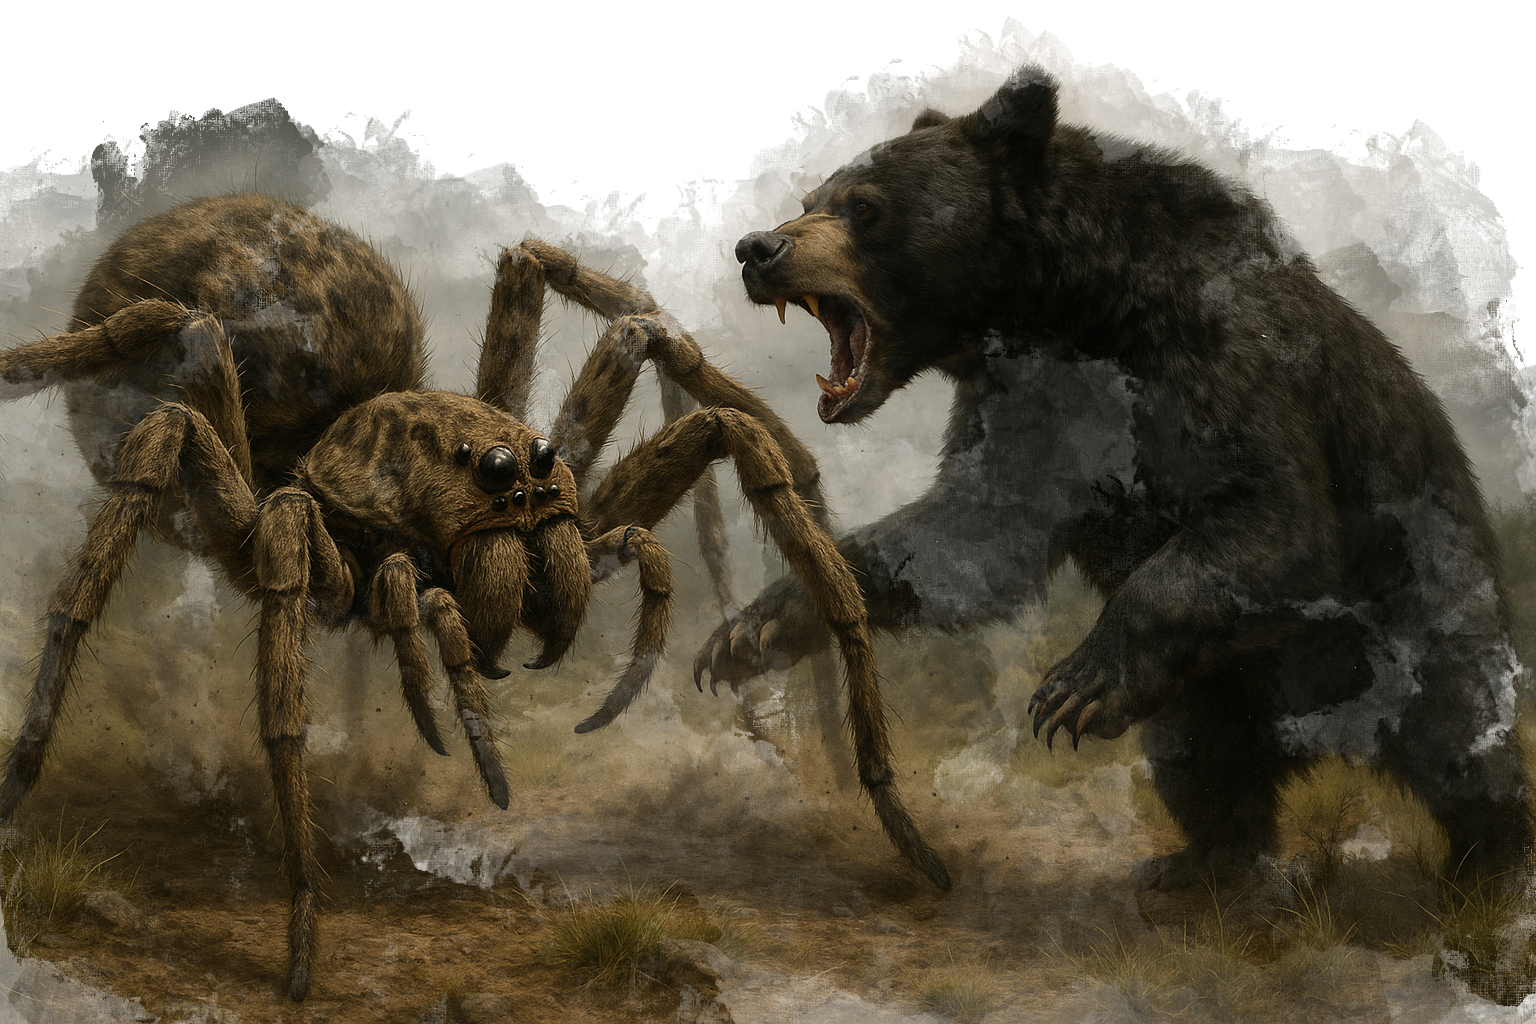
\includegraphics[width=\paperwidth]{Wolf_Spider_Black_Bear_background}%
      	\end{minipage}%
	};%
\end{tikzpicture}%
\vspace*{-2.7\fontdimen6\font}\hfill\\
\begin{DndMonster}[width=0.5\textwidth]{Giant Wolf Spider}
	\DndMonsterType{Medium Beast}
	
	\DndMonsterBasics[
		armor-class	= {13 (Natural Armor)},
		hit-points	= {\MaxHitPointsValue\ + \intcalcMul{1}{\LevelValue} temp HP},
		speed		= {50 ft., climb 50 ft.},
		initiative	= +3,
	]
	
	\renewcommand{\AbilityScoreSpacer}{~}
	
	\DndMonsterAbilityScores[
		str = 12,
		dex = 16,
		con = 13,
		int = 12,
		wis = 18,
		cha = 12,
	]
	
	\DndMonsterDetails[
		%saving-throws			= {},
		skills					= {Perception +\intcalcAdd{4}{\ProficiencyValue}, Stealth +\intcalcAdd{3}{\intcalcMul{2}{\ProficiencyValue}}},
		%damage-vulnerabilities	= {},
		%damage-resistances		= {cold},
		%damage-immunities		= {},
		%condition-immunities	= {},
		senses					= {Blindsight 10 ft., Darkvision 60 ft., Passive Perception \intcalcAdd{10}{\intcalcAdd{4}{\ProficiencyValue}}},
		languages				= -,
		challenge				= 1/4,
		proficiency-bonus		= \ProficiencyValue,
	]
	
	\DndMonsterSection{Traits}
	\DndMonsterAction{Spider Climb} The ice spider queen can climb difficult surfaces, including upside down on ceilings, without needing to make an ability check.
	
	\DndMonsterAction{Web Sense} While in contact with a web, the ice spider queen knows the exact location of any other creature in contact with the same web.
	
	\DndMonsterAction{Web Walker} The ice spider queen ignores movement restrictions caused by webbing.
	
	\DndMonsterSection{Actions}
	\DndMonsterAttack[
		name			= Bite,
		distance		= melee,
		%type			= weapon,
		mod				= +\intcalcAdd{1}{\ProficiencyValue},
		reach			= 5,
		%range			= 20/60,
		targets			= one target,
		dmg				= \DndDice{1d6 + 1},
		dmg-type		= piercing,
		%plus-dmg		= ,
		%plus-dmg-type	= ,
		%or-dmg			= ,
		%or-dmg-when	= ,
		extra			= {, and the target must make a DC 11 Constitution saving throw, taking \DndDice{2d6} poison damage on a failed save, or half as much damage on a successful one. If the poison damage reduces the target to 0 hit points, the target is stable but poisened for 1 hour, even after regaining hit points, and is paralyzed while poisened in this way},
	]
\end{DndMonster}
\vfill\eject
\section*{Black Bear}
\begin{DndMonster}[width=0.5\textwidth]{Black Bear}
	\DndMonsterType{Medium Beast}
	
	\DndMonsterBasics[
		armor-class	= {11 (Natural Armor)},
		hit-points	= {\MaxHitPointsValue\ + \intcalcMul{1}{\LevelValue} temp HP},
		speed		= {50 ft., climb 40 ft.},
		initiative	= +0,
	]
	
	\renewcommand{\AbilityScoreSpacer}{~}
	
	\DndMonsterAbilityScores[
		str = 15,
		dex = 10,
		con = 14,
		int = 10,
		wis = 18,
		cha = 18,
	]
	
	\DndMonsterDetails[
		%saving-throws			= {},
		skills					= {Perception +\intcalcAdd{4}{\ProficiencyValue}},
		%damage-vulnerabilities	= {},
		%damage-resistances		= {},
		%damage-immunities		= {},
		%condition-immunities	= {},
		senses					= {Passive Perception \intcalcAdd{10}{\intcalcAdd{4}{\ProficiencyValue}}},
		languages				= -,
		challenge				= 1/2,
		proficiency-bonus		= \ProficiencyValue,
	]
	
	\DndMonsterSection{Traits}
	\DndMonsterAction{Keen Smell} The bear has advantage on Wisdom (Perception) checks that rely on smell.
	
	\DndMonsterSection{Actions}
	\DndMonsterAction{Multiattack} The bear makes two attacks: one with its Bite an done with its Claws.
	
	\DndMonsterAttack[
		name			= Bite,
		distance		= melee,
		%type			= weapon,
		mod				= +\intcalcAdd{2}{\ProficiencyValue},
		reach			= 5,
		%range			= 20/60,
		targets			= one target,
		dmg				= \DndDice{1d6 + 2},
		dmg-type		= piercing,
		%plus-dmg		= ,
		%plus-dmg-type	= ,
		%or-dmg			= ,
		%or-dmg-when	= ,
		%extra			= {, },
	]
	\DndMonsterAttack[
		name			= Claw,
		distance		= melee,
		%type			= weapon,
		mod				= +\intcalcAdd{2}{\ProficiencyValue},
		reach			= 5,
		%range			= 20/60,
		targets			= one target,
		dmg				= \DndDice{2d4 + 2},
		dmg-type		= slashing,
		%plus-dmg		= ,
		%plus-dmg-type	= ,
		%or-dmg			= ,
		%or-dmg-when	= ,
		%extra			= {, },
	]
\end{DndMonster}
\vfill\eject
\section*{Ape}
\begin{tikzpicture}[overlay, remember picture, inner sep=0pt, outer sep=0pt, path fading=fade down]%
	\node[anchor=south west] at (current page.south west) {%
		\begin{minipage}{\paperwidth}%%
        	\centering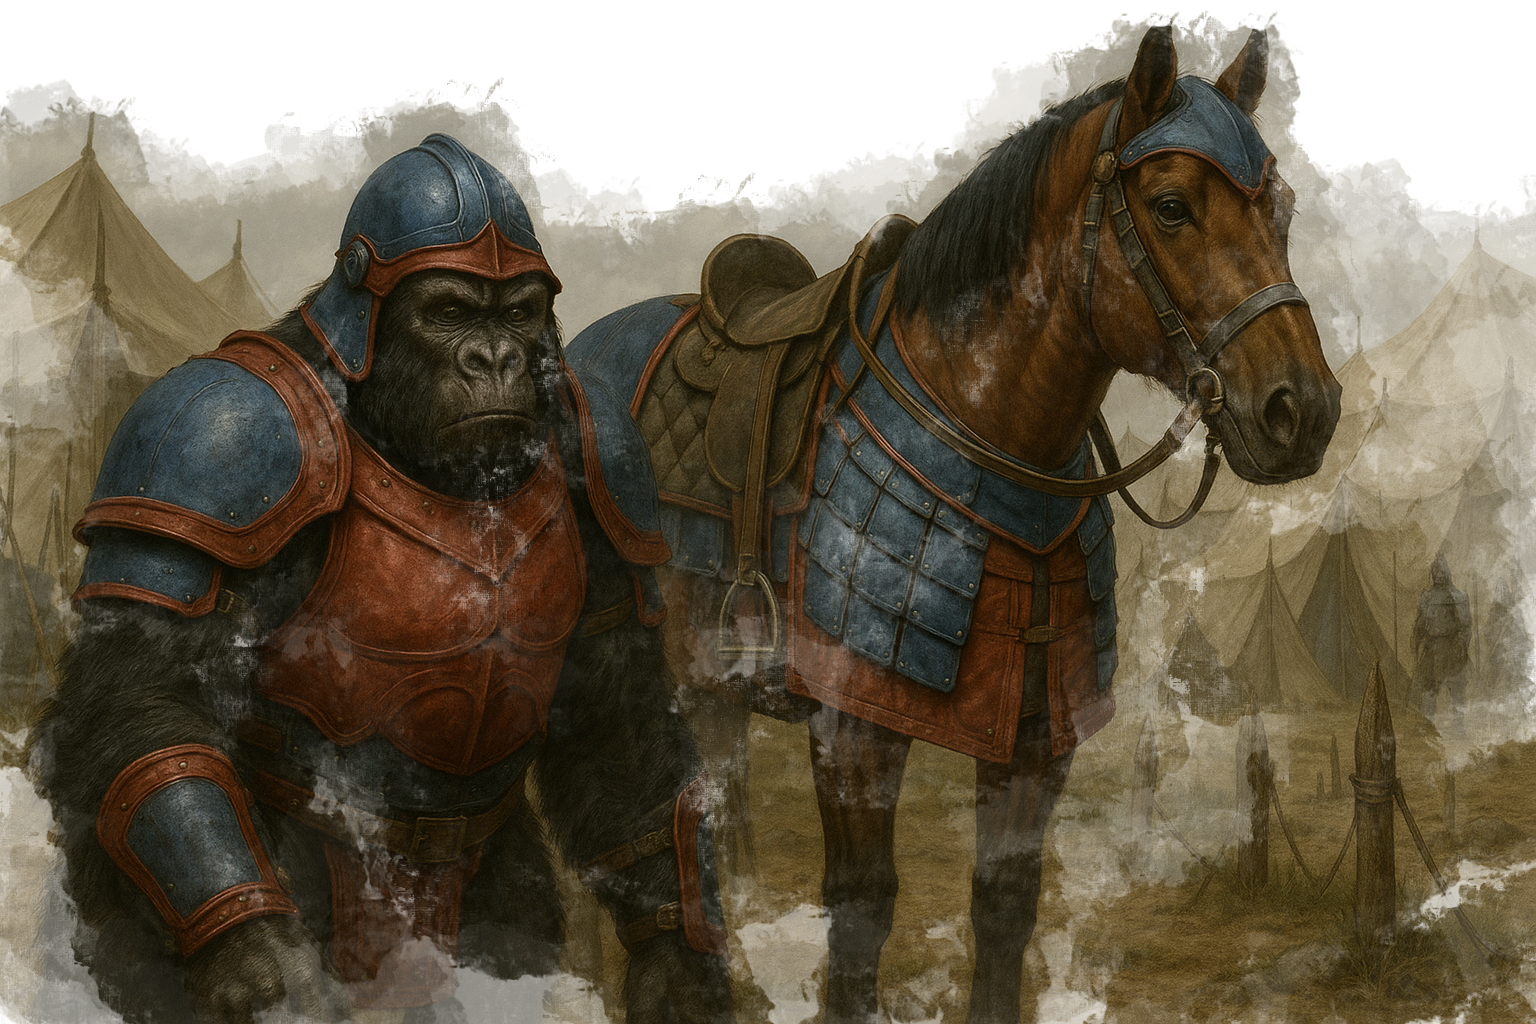
\includegraphics[width=\paperwidth]{Ape_Warhorse_background}%
      	\end{minipage}%
	};%
\end{tikzpicture}%
\vspace*{-2.7\fontdimen6\font}\hfill\\
\begin{DndMonster}[width=0.5\textwidth]{Ape}
	\DndMonsterType{Medium Beast}
	
	\DndMonsterBasics[
		armor-class	= {12 (Natural Armor)},
		hit-points	= {\MaxHitPointsValue\ + \intcalcMul{1}{\LevelValue} temp HP},
		speed		= {40 ft., climb 40 ft.},
		initiative	= +2,
	]
	
	\renewcommand{\AbilityScoreSpacer}{~}
	
	\DndMonsterAbilityScores[
		str = 16,
		dex = 14,
		con = 14,
		int = 10,
		wis = 18,
		cha = 18,
	]
	
	\DndMonsterDetails[
		%saving-throws			= {},
		skills					= {Athletics +\intcalcAdd{3}{\ProficiencyValue}, Perception +\intcalcAdd{4}{\ProficiencyValue}},
		%damage-vulnerabilities	= {},
		%damage-resistances		= {},
		%damage-immunities		= {},
		%condition-immunities	= {},
		senses					= {Passive Perception \intcalcAdd{10}{\intcalcAdd{4}{\ProficiencyValue}}},
		languages				= -,
		challenge				= 1/2,
		proficiency-bonus		= \ProficiencyValue,
	]
	
	\DndMonsterSection{Actions}
	\DndMonsterAction{Multiattack} The ape makes two fist attacks.
	
	\DndMonsterAttack[
		name			= Fist,
		distance		= melee,
		%type			= weapon,
		mod				= +\intcalcAdd{3}{\ProficiencyValue},
		reach			= 5,
		%range			= 20/60,
		targets			= one target,
		dmg				= \DndDice{1d6 + 3},
		dmg-type		= bludgeoning,
		%plus-dmg		= ,
		%plus-dmg-type	= ,
		%or-dmg			= ,
		%or-dmg-when	= ,
		%extra			= {, },
	]
	\DndMonsterAttack[
		name			= Stone,
		distance		= ranged,
		%type			= weapon,
		mod				= +\intcalcAdd{3}{\ProficiencyValue},
		%reach			= 5,
		range			= 25/50,
		targets			= one target,
		dmg				= \DndDice{1d6 + 3},
		dmg-type		= bludgeoning,
		%plus-dmg		= ,
		%plus-dmg-type	= ,
		%or-dmg			= ,
		%or-dmg-when	= ,
		%extra			= {, },
	]
\end{DndMonster}
\vfill\eject
\section*{Warhorse}
\begin{DndMonster}[width=0.5\textwidth]{Warhorse}
	\DndMonsterType{Large Beast}
	
	\DndMonsterBasics[
		armor-class	= {11 (Natural Armor)},
		hit-points	= {\MaxHitPointsValue\ + \intcalcMul{1}{\LevelValue} temp HP},
		speed		= {70 ft.},
		initiative	= +1,
	]
	
	\renewcommand{\AbilityScoreSpacer}{~}
	
	\DndMonsterAbilityScores[
		str = 18,
		dex = 12,
		con = 13,
		int = 10,
		wis = 18,
		cha = 18,
	]
	
	\DndMonsterDetails[
		%saving-throws			= {},
		skills					= {Perception +\intcalcAdd{4}{\ProficiencyValue}},
		%damage-vulnerabilities	= {},
		%damage-resistances		= {},
		%damage-immunities		= {},
		%condition-immunities	= {},
		senses					= {Passive Perception \intcalcAdd{10}{\intcalcAdd{4}{\ProficiencyValue}}},
		languages				= -,
		challenge				= 1/2,
		proficiency-bonus		= \ProficiencyValue,
	]
	
	\DndMonsterSection{Traits}
	\DndMonsterAction{Trampling Charge} If the horse moves at least 20 feet straight toward a creature and then hits it with a hooves attack on the same turn, that target must succeed on a DC 14 Strength saving throw or be knocked prone. If the target is prone, the horse can make another attack with its hooves against it as a bonus action.
	
	\DndMonsterSection{Actions}
	\DndMonsterAttack[
		name			= Hooves,
		distance		= melee,
		%type			= weapon,
		mod				= +\intcalcAdd{4}{\ProficiencyValue},
		reach			= 5,
		%range			= 20/60,
		targets			= one target,
		dmg				= \DndDice{2d6 + 4},
		dmg-type		= bludgeoning,
		%plus-dmg		= ,
		%plus-dmg-type	= ,
		%or-dmg			= ,
		%or-dmg-when	= ,
		%extra			= {, },
	]
\end{DndMonster}
\vfill\eject
\section*{Giant Sea Horse}
\begin{tikzpicture}[overlay, remember picture, inner sep=0pt, outer sep=0pt, path fading=fade down]%
	\node[anchor=south west] at (current page.south west) {%
		\begin{minipage}{\paperwidth}%%
        	\centering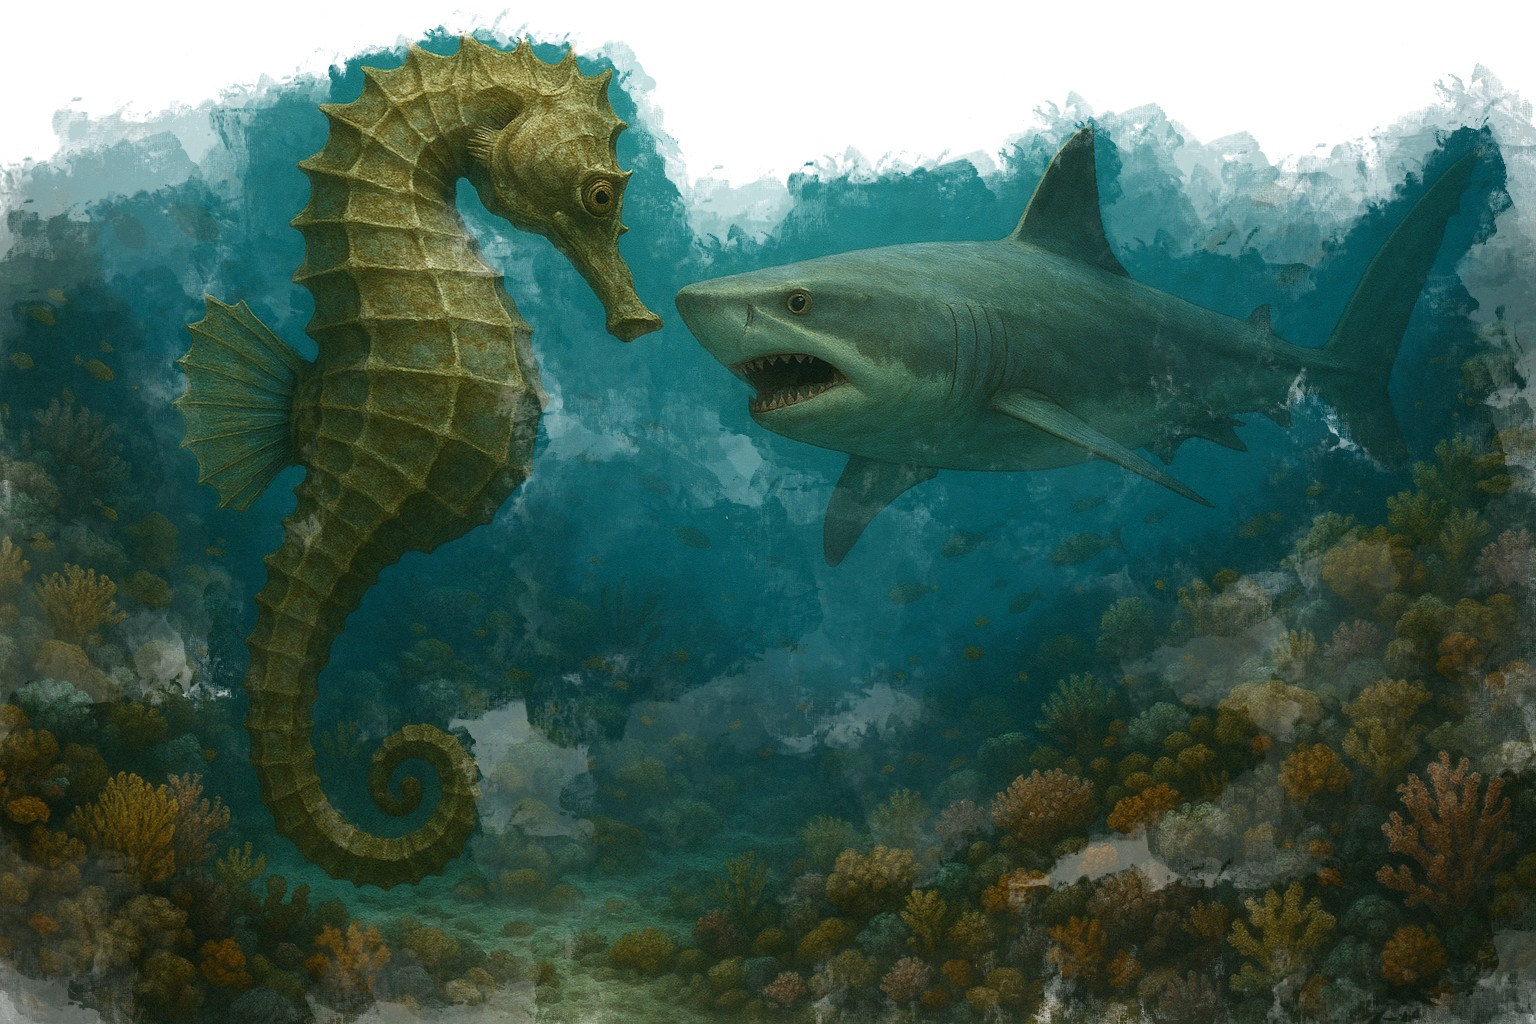
\includegraphics[width=\paperwidth]{Sea_Horse_Shark_background}%
      	\end{minipage}%
	};%
\end{tikzpicture}%
\vspace*{-2.7\fontdimen6\font}\hfill\\
\begin{DndMonster}[width=0.5\textwidth]{Giant Sea Horse}
	\DndMonsterType{Large Beast}
	
	\DndMonsterBasics[
		armor-class	= {14 (Natural Armor)},
		hit-points	= {\MaxHitPointsValue\ + \intcalcMul{1}{\LevelValue} temp HP},
		speed		= {10 ft., swim 50 ft.},
		initiative	= +2,
	]
	
	\renewcommand{\AbilityScoreSpacer}{~}
	
	\DndMonsterAbilityScores[
		str = 12,
		dex = 15,
		con = 11,
		int = 10,
		wis = 18,
		cha = 18,
	]
	
	\DndMonsterDetails[
		%saving-throws			= {},
		skills					= {Perception +\intcalcAdd{4}{\ProficiencyValue}},
		%damage-vulnerabilities	= {},
		%damage-resistances		= {},
		%damage-immunities		= {},
		%condition-immunities	= {},
		senses					= {Passive Perception \intcalcAdd{10}{\intcalcAdd{4}{\ProficiencyValue}}},
		languages				= -,
		challenge				= 1/2,
		proficiency-bonus		= \ProficiencyValue,
	]
	
	\DndMonsterSection{Traits}
	\DndMonsterAction{Charge} If the sea horse moves at least 20 feet straight toward a target and then hits it with a ram attack on the same turn, the target takes an extra \DndDice{2d6} bludgeoning damage. It the target is a creature, it must succeed on a DC 11 Strength saving throw or be knocked prone.
	
	\DndMonsterAction{Water Breathing} The sea horse can breathe only underwater.
	
	\DndMonsterSection{Actions}
	\DndMonsterAttack[
		name			= Ram,
		distance		= melee,
		%type			= weapon,
		mod				= +\intcalcAdd{1}{\ProficiencyValue},
		reach			= 5,
		%range			= 20/60,
		targets			= one target,
		dmg				= \DndDice{1d6 + 1},
		dmg-type		= bludgeoning,
		%plus-dmg		= ,
		%plus-dmg-type	= ,
		%or-dmg			= ,
		%or-dmg-when	= ,
		%extra			= {, },
	]
\end{DndMonster}
\vfill\eject
\section*{Reef Shark}
\begin{DndMonster}[width=0.5\textwidth]{Reef Shark}
	\DndMonsterType{Medium Beast}
	
	\DndMonsterBasics[
		armor-class	= {12 (Natural Armor)},
		hit-points	= {\MaxHitPointsValue\ + \intcalcMul{1}{\LevelValue} temp HP},
		speed		= {10 ft., swim 50 ft.},
		initiative	= +1,
	]
	
	\renewcommand{\AbilityScoreSpacer}{~}
	
	\DndMonsterAbilityScores[
		str = 14,
		dex = 13,
		con = 13,
		int = 10,
		wis = 18,
		cha = 18,
	]
	
	\DndMonsterDetails[
		%saving-throws			= {},
		skills					= {Perception +\intcalcAdd{4}{\ProficiencyValue}},
		%damage-vulnerabilities	= {},
		%damage-resistances		= {},
		%damage-immunities		= {},
		%condition-immunities	= {},
		senses					= {Passive Perception \intcalcAdd{10}{\intcalcAdd{4}{\ProficiencyValue}}},
		languages				= -,
		challenge				= 1/2,
		proficiency-bonus		= \ProficiencyValue,
	]
	
	\DndMonsterSection{Traits}
	\DndMonsterAction{Pack Tactics} The shark has advantage on an attack roll against a creature if at least one of the shark's allies is within 5 feet of the creature and the ally isn't incapacitated.
	
	\DndMonsterAction{Water Breathing} The sea horse can breathe only underwater.
	
	\DndMonsterSection{Actions}
	\DndMonsterAttack[
		name			= Bite,
		distance		= melee,
		%type			= weapon,
		mod				= +\intcalcAdd{2}{\ProficiencyValue},
		reach			= 5,
		%range			= 20/60,
		targets			= one target,
		dmg				= \DndDice{1d8 + 2},
		dmg-type		= piercing,
		%plus-dmg		= ,
		%plus-dmg-type	= ,
		%or-dmg			= ,
		%or-dmg-when	= ,
		%extra			= {, },
	]
\end{DndMonster}
\end{document}